\documentclass{masterthesis}
% masterthesis for Computer Science
% masterthesis_ceng for Computer Engineering
% use the [nocoverpage] option to speed up compilation by skipping the cover page

% the configuration is in the preamble.tex file, read it and modify it to change
% the document appearance and included packages
% we use biblatex, which is a more modern alternative to the traditional bibtex
% comment this to use bibtex instead
\usepackage[
    backend=biber,
    style=alphabetic,
    sorting=nyt,
    maxbibnames=99
]{biblatex}

% graphicx is needed to include images
\usepackage{graphicx}
\usepackage{adjustbox}
\usepackage{float}
\usepackage{flafter} % a figure never appears before the text that introduces it
% let large figures share a page with text and with each other (less empty space)
\renewcommand{\topfraction}{0.85}
\renewcommand{\bottomfraction}{0.7}
\renewcommand{\textfraction}{0.1}
\renewcommand{\floatpagefraction}{0.75}

% xspace is used to add a space after a macro, if needed
\usepackage{xspace}

% acronym (https://ctan.org/pkg/acronym) is a package to expand acronyms after their first usage
\usepackage{acronym}

% the hyperref package provides links; with this configuration they are colored
% according to the scheme described in https://tex.stackexchange.com/a/525297
\usepackage{xcolor}
\usepackage[colorlinks]{hyperref}
\def\tmp#1#2#3{%
  \definecolor{Hy#1color}{#2}{#3}%
  \hypersetup{#1color=Hy#1color}}
\tmp{link}{HTML}{800006}
\tmp{cite}{HTML}{2E7E2A}
\tmp{file}{HTML}{131877}
\tmp{url} {HTML}{8A0087}
\tmp{menu}{HTML}{727500}
\tmp{run} {HTML}{137776}
\def\tmp#1#2{%
  \colorlet{Hy#1bordercolor}{Hy#1color#2}%
  \hypersetup{#1bordercolor=Hy#1bordercolor}}
\tmp{link}{!60!white}
\tmp{cite}{!60!white}
\tmp{file}{!60!white}
\tmp{url} {!60!white}
\tmp{menu}{!60!white}
\tmp{run} {!60!white}

% the cleveref package is used to automatically add the type of reference
% (e.g., "section", "figure", "table") to the reference using the \cref command
% The "capitalize" option makes both \cref and \Cref uppercase; if we remove it
% only \Cref will be uppercase.
\usepackage[capitalize]{cleveref}
% cleveref loads before listings below, so it does not know what to call an
% \lstlisting by default; name it explicitly or \Cref{lst:...} prints "??"
\crefname{lstlisting}{Listing}{Listings}
\Crefname{lstlisting}{Listing}{Listings}

% the booktabs package is used to create better tables; check an example of usage in results.tex
\usepackage{booktabs}
\usepackage{tabularx}

% breaks long URLs better
\usepackage{xurl}

% macros
\newcommand*{\latex}{\LaTeX \xspace}
\newcommand{\myhref}[2]{#2\footnote{\url{#1}}}

% tracking changes using the todonotes package
\setlength{\marginparwidth}{2cm}
\usepackage{todonotes}
\newcommand{\note}[3]{\todo[inline,color=#2]{#1: #3}}
\newcommand{\md}[1]{\note{MD}{yellow}{#1}}

% result is something like "Related Work (Chapter 2)"
\newcommand{\fullref}[1]{\nameref{#1} (\Cref{#1})}

% used for the inparaenum environment
\usepackage{paralist}

% code listings for chaincode and API examples
\usepackage{listings}
\usepackage{lstautogobble}
\lstset{
    basicstyle=\ttfamily\small,
    breaklines=true,
    frame=single,
    numbers=left
}

% for nicer diagrams and architecture figures
\usepackage{tikz}
\usetikzlibrary{arrows.meta,positioning,fit,calc}

% styles shared by the TikZ figures
\tikzset{
    box/.style={draw, rounded corners=2pt, align=center, minimum height=9mm, inner sep=4pt, fill=gray!8},
    chain/.style={draw, rounded corners=2pt, align=center, minimum height=9mm, minimum width=22mm, inner sep=3pt, fill=blue!6},
    arr/.style={-{Latex[length=2mm]}, thick},
    darr/.style={-{Latex[length=2mm]}, thick, dashed},
    lbl/.style={font=\scriptsize, midway, fill=white, inner sep=1pt}
}

% \screenshot{file}{caption}{label}: includes images/<file> when it exists,
% otherwise draws a labelled placeholder so the document still compiles.
% Use file names without underscores.
% Screenshots never appear before the text that introduces them (flafter). \screenshot uses the full text width; \modalshot crops
% the blurred background around a window (about 23.5% left/right, 4% top/bottom)
% so that the window itself fills the width.
\newcommand{\modalshot}[3]{%
    \begin{figure}[!htbp]
        \centering
        \IfFileExists{#1}%
            {\adjustbox{trim={.235\width} {.04\height} {.235\width} {.04\height},clip,width=0.66\textwidth}{\includegraphics{#1}}}%
            {\fbox{\parbox{0.8\textwidth}{\centering\vspace{2.2cm}\texttt{#1}\\[2pt]\small screenshot to be added\vspace{2.2cm}}}}
        \caption{#2}
        \label{#3}
    \end{figure}}
\newcommand{\screenshot}[3]{%
    \begin{figure}[!htbp]
        \centering
        \IfFileExists{#1}%
            {\includegraphics[width=\textwidth]{#1}}%
            {\fbox{\parbox{0.8\textwidth}{\centering\vspace{2.2cm}\texttt{#1}\\[2pt]\small screenshot to be added\vspace{2.2cm}}}}
        \caption{#2}
        \label{#3}
    \end{figure}}

% Anita's own notes
\newcommand{\ag}[1]{\note{AG}{cyan}{#1}}

% by default, we use the biblatex package to manage the bibliography
% if you prefer to use bibtex, comment the following line and uncomment the
% relevant lines at the end of the document
\addbibresource{bib.bib}

\acrodef{DIBRIS}{\textit{dipartimento di informatica, bioingegneria, robotica e ingegneria dei sistemi}}
\acrodef{LLM}{large language model}


\begin{document}

\title{Decentralized Project Management System with Blockchain and IPFS}

\author{Anita Ghezel Ayagh Tehrani}

\advisor{Marina Ribaudo}

\examiner{Gianna Reggio}

\submitmonth{December}
\submityear{2026}

\maketitle

\begin{abstract}
Software project management platforms in wide use today, such as Trello, Jira, Asana, GitHub Projects and GitLab, share a common limitation: the history of changes to a project is stored and controlled entirely by a single centralized provider, with no mechanism for participants to verify independently that it has not been altered. This thesis proposes and implements a decentralized project management system that addresses this limitation by combining Hyperledger Fabric, a permissioned blockchain framework, with the InterPlanetary File System (IPFS) for off-chain file storage.

The system, named ChainBoard, models accounts, projects and tasks as chaincode-governed state on a Fabric ledger, and every change is permanently recorded in an immutable transaction history. The chaincode itself enforces who may do what, according to the roles of owner, administrator and contributor, so that the permission rules do not depend on the backend or the user interface. Files attached to tasks are stored on IPFS and referenced on-chain by their content identifiers. A browser frontend offers a familiar task board, and a verification procedure checks every record of a history against the ledger and produces a downloadable report with a digest chain that can be verified again offline.

The prototype was evaluated on a real Fabric network with functional scenarios, permission tests for every role, deliberate manipulations of audit reports, 278 automated tests, a benchmark and a user study. All scenarios passed, every forbidden action was refused by the chaincode, and every manipulation was detected. A write takes about 2 seconds, mostly waiting for a block, and a read about 30 milliseconds. In a user study with ten participants, everyone completed all twelve tasks, and the System Usability Scale score was 86 out of 100, well above the usual average of 68.
\end{abstract}

\tableofcontents

\chapter{Introduction}
\label{ch:introduction}

\section{Motivation}
\label{sec:motivation}

Software teams plan and track their work in tools such as Trello, Jira, Asana, GitHub Projects or GitLab. These tools work well, but in all of them one company stores every task, every status change and every log of who did what. If a team wants to be sure that the history of a task has not been changed, it can only trust the provider. There is no way to check.

Most of the time this is fine. It becomes a problem when the people working on a project do not fully trust each other, or when they must be able to prove later who did what and when. Examples are projects shared by several companies, outsourced development, and academic or regulated work where accountability has to be shown, not just claimed.

Permissioned blockchains such as Hyperledger Fabric were built for this situation: a known group of organizations shares a record of changes that none of them can rewrite alone. \textcite{adel2023} used Fabric together with the InterPlanetary File System (IPFS) to manage shared data in construction projects, keeping metadata on the ledger and documents on IPFS. Their data model, however, is made for construction sites, not for software teams.

In this thesis I take the same Fabric and IPFS approach and apply it to software project management. The result, ChainBoard, looks like a normal task board, with projects, tasks, priorities, assignments, comments and file attachments, but its history is stored on a ledger and every user can verify it.

\section{Research Questions}
\label{sec:rqs}

\begin{description}
    \item[RQ1] Can the Fabric and IPFS approach used for construction data be adapted to software project management, with the functions teams expect from tools like Trello or Jira?
    \item[RQ2] Can the rules of who may do what in a project be enforced by the chaincode itself, so that they do not depend on the backend or the user interface?
    \item[RQ3] How can the history of a task or project be made tamper-evident, and checkable by a person who has no access to the blockchain network?
    \item[RQ4] What does this cost in speed, and where are its limits?
\end{description}

\section{Contributions}
\label{sec:contributions}

The thesis makes four contributions:
\begin{enumerate}
    \item a data model and chaincode for accounts, projects and tasks on Hyperledger Fabric, with file attachments on IPFS;
    \item role-based permissions checked by the chaincode on every change;
    \item an audit check that compares each record of a history with the ledger and produces a report with a digest chain that can be verified offline;
    \item an evaluation with functional tests, a benchmark and a threat model.
\end{enumerate}

\section{Structure of the Thesis}
\label{sec:content}

\Cref{ch:background} explains the concepts used later: project management and agile methods, blockchains, Hyperledger Fabric and IPFS. \Cref{ch:related} discusses similar systems and where ChainBoard differs from them. \Cref{ch:method} describes the design and implementation, \Cref{ch:results} the evaluation, and \Cref{ch:conclusion} answers the research questions and lists the limitations and future work. The appendix explains how to run the prototype and repeat the measurements.


\chapter{Background}
\label{ch:background}

\section{Project Management}
\label{sec:pm}

Project management is the work of organizing tasks, people and resources to reach a goal within limits of time, budget and quality~\cite{pmbok}. A project usually goes through five phases: initiation, where the goal and the people involved are defined; planning, where the work is split into tasks with owners and deadlines; execution; monitoring, where progress is compared with the plan; and closing, where the result is delivered and the project archived.

For a software team, a project management tool must at least let people create and assign tasks, follow their status, control who can do what, attach files, comment, and see the history of changes. These are the requirements ChainBoard is built around.

\section{Current Tools and Their Limits}
\label{sec:traditional-pm}

Trello organizes work as cards on a board, an idea taken from Kanban. Jira, the most common tool in professional software development, adds backlogs, sprints, epics and reports, and is powerful but complex to set up. Asana focuses on coordination across many projects. GitHub Projects and GitLab connect tasks to the code, which makes them natural for developers.

They differ in features, but they share one design: a single provider stores all the data and decides who can see and change it. This has three consequences. First, there is no history that others can check independently; audit logs exist, but the provider controls them. Second, organizations do not control where their data is kept. Third, if the service goes down or is discontinued, every team that depends on it is affected. The first point is the one this thesis addresses.

\section{Agile Methods: Scrum and Kanban}
\label{sec:agile}

Most software teams work iteratively. In Scrum~\cite{scrumguide2020}, work is done in sprints of at most one month. The Product Owner orders the product backlog, the developers build an increment of the product in each sprint, and the Scrum Master helps the team follow the method. Each sprint starts with planning and ends with a review of the result and a retrospective on how the team worked. Kanban~\cite{anderson2010kanban} has no sprints or roles: the work is shown on a board whose columns are the stages of the work, and the team limits how many items are in progress at once.

Both methods depend on a shared and reliable view of the work: which tasks exist, who is working on them and in which stage they are. This is exactly the information ChainBoard protects.

\section{Blockchain}
\label{sec:blockchain}

A blockchain is a ledger copied across many nodes, in which each block contains the hash of the previous one~\cite{nakamoto2008bitcoin}. Changing an old block would change every block after it, so a change cannot go unnoticed. Public blockchains such as Bitcoin and Ethereum let anyone join and use expensive consensus mechanisms. Permissioned blockchains only accept known, authenticated members and can use cheaper protocols, which makes them suitable for companies.

A blockchain is not always the right choice. \textcite{wust2018need} suggest asking whether several parties write the data, whether they trust each other, and whether a trusted third party is available. For one team that trusts its own administrator, a normal database is simpler and faster. For several organizations that share a project and want a history none of them can rewrite, a permissioned blockchain fits. This thesis is about the second case.

The programs that run on a blockchain and define how its state may change are called smart contracts. Because the network runs them, no single participant can change the rules alone.

\section{Hyperledger Fabric}
\label{sec:fabric}

Hyperledger Fabric~\cite{androulaki2018} is an open-source permissioned blockchain. The parts that matter for this thesis are:

\begin{description}
    \item[Organizations and peers.] Each organization runs one or more peers, and each peer keeps a copy of the ledger.
    \item[Orderer.] It puts transactions into blocks and sends the blocks to the peers.
    \item[Channel.] A ledger shared by a group of organizations.
    \item[Chaincode.] Fabric's name for smart contracts, written in Go, JavaScript or Java.
    \item[World state and history.] The world state holds the current value of each key. The history holds every earlier value and cannot be changed, so it works as a permanent log.
    \item[Identities.] Every participant has an X.509 certificate issued by its organization.
    \item[Endorsement.] Before a transaction is ordered, the endorsing peers run it and must get exactly the same result. When two transactions in one block change the same key, only the first is accepted and the other fails with a read conflict.
\end{description}

I chose Fabric over Ethereum because the participants of a project are known, no fees or wallets are needed, and data can be kept private between organizations if necessary.

\section{Hash Chains}
\label{sec:hash-chains}

A log is tamper-evident if changes to it can be detected, even when they cannot be prevented. The usual technique is a hash chain~\cite{schneier1999secure}: each entry is hashed together with the hash of the entry before it. If an entry is changed, removed, added or moved, every hash after it changes, so the last hash is a short fingerprint of the whole log. A blockchain is a hash chain shared by many nodes. ChainBoard also builds a small hash chain over the history of one task, so that a user can keep its fingerprint and check it later (\Cref{sec:audit-verification}).

\section{IPFS}
\label{sec:ipfs}

The InterPlanetary File System (IPFS)~\cite{benet2014ipfs} is a peer-to-peer file system that finds files by their content instead of their location. A file is hashed, and the hash, called a content identifier (CID), is its address. If the file changes, its CID changes too, so a CID stored on a ledger proves exactly which file was attached. Files can be fetched from any node that has a copy. Storing large files directly on a blockchain is slow and expensive, so the usual approach, which ChainBoard follows, is to keep the file on IPFS and only its CID on the ledger.


\chapter{Related Work}
\label{ch:related}

\section{Fabric and IPFS in Construction}
\label{sec:adel}

The work closest to this thesis is the system of \textcite{adel2023} for construction projects. A construction project involves several independent companies, such as contractors, architects and engineers, who share task data and documents and need a record of changes that no single party controls. Adel et al.\ store task and progress records on Hyperledger Fabric and large files such as drawings and reports on IPFS, with only the CID kept on the ledger. They also use Fabric channels and private data to limit what each party can see.

ChainBoard follows the same split between on-chain metadata and off-chain files. The difference is the domain. A construction task is a physical milestone with drawings and permits, while a software task is an issue with a priority, an assignee and a short to-do, in-progress, done workflow. Software teams are also used to tools like Jira and expect a similar interface. These differences shape the data model and the user interface of ChainBoard.

\section{Blockchain-Based Project Management}
\label{sec:related-pm}

Reviews of the field find that blockchain is used in project management mostly where several parties must coordinate and check each other's work, and that outside construction most systems are still prototypes~\cite{noteboom2026coordination}. Three systems are close to ChainBoard.

\textcite{batista2021} built a project management tool on Hyperledger Fabric in a master's thesis. Its chaincode handles projects, users, tasks with dependencies, timesheets and an automatic risk analysis, and every user has their own Fabric identity. It offers an API but no user interface, and users cannot verify a history themselves. In load tests on one laptop it reached at most 41.6 write and 159.1 read transactions per second.

Scrum-Chain~\cite{silva_scrumchain} records the Scrum cycle (backlog, sprints and tasks) in Solidity contracts on an Ethereum test network. Users sign every action with the MetaMask wallet, and the data is also copied to a PostgreSQL database, which the interface reads. It is one of the few such systems tested with users: ten student teams used it for several sprints, rated it positively and named the audit trail as its most useful feature, while the wallet was the main source of problems.

ChainAgile~\cite{qureshi2024chainagile} supports distributed Scrum teams on a private Ethereum network, with contracts for user stories, acceptance tests and payments, and IPFS for files.

\section{Tamper-Evident Audit Logs}
\label{sec:related-logging}

Blockchains have also been used just to protect audit logs. BlockAudit~\cite{ahmad2018blockaudit}, for example, turns the entries of a normal audit log into transactions on Hyperledger. In such systems the log is separate from the data it describes. In ChainBoard the ledger is the only place where the project data is stored, so the history and the data cannot drift apart.

\section{Positioning}
\label{sec:positioning}

\Cref{tab:related} compares ChainBoard with the systems above. ChainBoard is not the most complete of them: it has no sprints, and unlike Batista's tool it does not give every person a Fabric identity. What it adds is the combination of a familiar board interface without wallets or fees, permissions checked by the chaincode, the ledger as the only data store, and an audit check that ordinary users can run and repeat offline.

\begin{table}[!htb]
    \centering
    \small
    \setlength{\tabcolsep}{4pt}
    \begin{tabular}{llcccc}
        \toprule
        System & Platform & \shortstack{User\\interface} & \shortstack{No wallet\\needed} & \shortstack{Ledger is the\\only store} & \shortstack{Users can\\verify history} \\
        \midrule
        Adel et al.~\cite{adel2023} & Fabric + IPFS & no (CLI) & yes & yes & no \\
        Batista~\cite{batista2021} & Fabric & no & yes & yes & no \\
        Scrum-Chain & Ethereum & yes & no & no & no \\
        ChainAgile & Ethereum + IPFS & yes & no & yes & no \\
        ChainBoard & Fabric + IPFS & yes & yes & yes & yes \\
        \bottomrule
    \end{tabular}
    \caption{ChainBoard compared with related systems.}
    \label{tab:related}
\end{table}


\chapter{System Design and Implementation}
\label{ch:method}

\section{Architecture}
\label{sec:architecture}

ChainBoard has four parts (\Cref{fig:architecture}):

\begin{enumerate}
    \item a \textbf{frontend} in the browser, built with React and Vite, where people sign in and work with projects and tasks;
    \item a \textbf{backend} in Node.js and Express, which checks who is signed in and turns HTTP requests into Fabric transactions;
    \item a \textbf{Hyperledger Fabric network} with two organizations, one peer each, one orderer and one channel, where the chaincode stores the data and checks every rule;
    \item an \textbf{IPFS node} that stores attached files.
\end{enumerate}

\begin{figure}[tb]
    \centering
    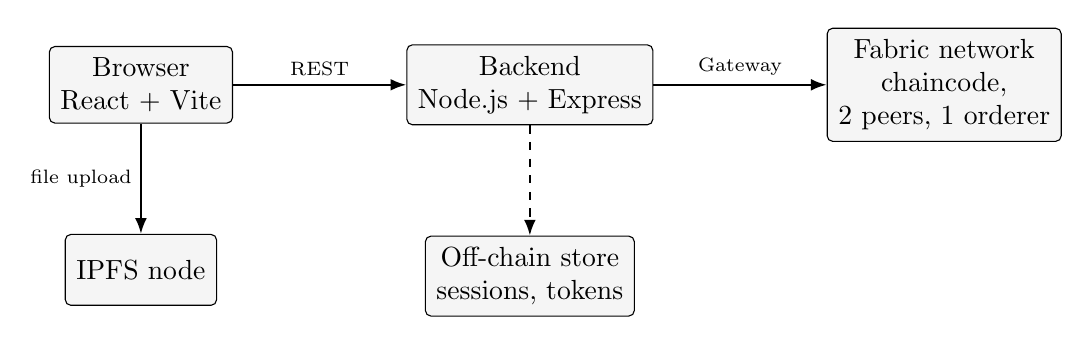
\begin{tikzpicture}[node distance=14mm and 22mm]
        \node[box] (fe) {Browser\\ React + Vite};
        \node[box, right=of fe] (be) {Backend\\ Node.js + Express};
        \node[box, right=of be] (fab) {Fabric network\\ chaincode,\\ 2 peers, 1 orderer};
        \node[box, below=of fe] (ipfs) {IPFS node};
        \node[box, below=of be] (store) {Off-chain store\\ sessions, tokens};
        \draw[arr] (fe) -- node[lbl, above=2pt, fill=none] {REST} (be);
        \draw[arr] (be) -- node[lbl, above=2pt, fill=none] {Gateway} (fab);
        \draw[arr] (fe) -- node[lbl, left=2pt, fill=none] {file upload} (ipfs);
        \draw[darr] (be) -- (store);
    \end{tikzpicture}
    \caption{Architecture of ChainBoard. The browser talks only to the backend, except when it uploads a file to IPFS. Only the backend holds the organization's Fabric identity.}
    \label{fig:architecture}
\end{figure}

Everything with business meaning, including user accounts, is on the ledger. The backend keeps only short-lived data off the chain: login sessions, e-mail confirmation tokens and rate-limit counters.

When a user creates a task, the frontend sends a request to the backend. The backend finds the signed-in user from the session cookie and submits a transaction through the Fabric Gateway, passing that user as the person who acts. Both peers endorse the transaction, the orderer puts it in a block, and both peers commit it. The backend then returns the new task as JSON. Reads use \texttt{evaluateTransaction}, which asks one peer and does not create a block. Attaching a file adds one step: the browser first uploads the file to IPFS, gets its CID, and then sends only the CID and the file name to the backend.

\section{Chaincode}
\label{sec:chaincode-design}

The chaincode is written in JavaScript. It stores three kinds of records, users, projects and tasks, each under its own key. Every time a key is written, Fabric also adds the new value to that key's history.

\paragraph*{Data model.} A project has a name, a description, an owner, a list of members with their role (\texttt{owner}, \texttt{admin} or \texttt{contributor}) and a status (\texttt{active} or \texttt{archived}). A task belongs to a project and has a title, a description, a priority, an optional due date, a status (\texttt{todo}, \texttt{in-progress} or \texttt{done}), an optional assignee, an archived flag, attachments and comments. Projects and tasks also store \texttt{updatedBy}, so every version in the history says who made it.

\paragraph*{Keys.} Fabric's default database, LevelDB, can look up a key or scan a range of keys, but it cannot search by field. So the keys are the design: \texttt{project:<id>}, \texttt{task:<id>} and \texttt{user:<email>}, plus index keys such as \texttt{idx:username:<name>} that make usernames unique. The tasks of a project are found by scanning the \texttt{task:} keys. This way the board can always be rebuilt from the ledger.

\paragraph*{Functions.} The project functions create a project, add a member, archive the project, list its tasks and return its history. The task functions create, assign, move, edit, comment, attach a file, archive and return the history. Only some status moves are allowed: \texttt{todo} to \texttt{in-progress}, \texttt{in-progress} back to \texttt{todo} or on to \texttt{done}, and a finished task can be reopened. A task cannot jump from \texttt{todo} to \texttt{done}, and every reopening stays visible. A ledger cannot delete anything, so archiving only hides a task or project from the board while its history remains.

\subsection{Permissions}
\label{sec:permissions}

The chaincode, not the backend or the interface, decides who may do what. Every function that changes data receives the person who acts as its last argument and checks that person's role in the project record. \Cref{tab:permissions} shows the rules.

\begin{table}[htbp]
    \centering
    \small
    \begin{tabular}{p{4.2cm}p{2.1cm}p{2.1cm}p{3.3cm}}
        \toprule
        Action & Owner & Admin & Contributor \\
        \midrule
        Add a member & any role & contributors only & no \\
        Archive the project & yes & no & no \\
        Create a task, comment & yes & yes & yes \\
        Assign a task & anyone & anyone & only to themselves, if the task is free \\
        Change status, edit, attach a file & any task & any task & own or unassigned tasks \\
        Archive a task & yes & yes & no \\
        \bottomrule
    \end{tabular}
    \caption{Permissions checked by the chaincode. People outside the project can do none of these.}
    \label{tab:permissions}
\end{table}

Listing~\ref{lst:permissions} shows the helper functions and the check in \texttt{addProjectMember}; the other functions start with a similar check.

\begin{lstlisting}[caption={Role helpers and the check in \texttt{addProjectMember} (simplified).}, label={lst:permissions}, numbers=none, basicstyle=\ttfamily\footnotesize, language={}, autogobble]
    function roleOf(project, id) {
        const found = (project.members || []).find(m => m.id === id);
        return found ? found.role : null;
    }
    function isManager(role) { return role === 'owner' || role === 'admin'; }
    function canWorkOnTask(role, task, actorId) {
        if (!role) return false;
        return isManager(role) || !task.assigneeId || task.assigneeId === actorId;
    }

    // inside addProjectMember(projectId, memberId, role, actorId)
    const actorRole = roleOf(project, actorId);
    if (!isManager(actorRole))
        return shim.error('Permission denied: only project owners and admins can add members');
    if (actorRole === 'admin' && role !== 'contributor')
        return shim.error('Permission denied: admins can only add contributors');
\end{lstlisting}

The backend turns ``Permission denied'' into HTTP 403. The interface uses the same rules to grey out buttons and explain why, but that is only for convenience: if someone calls the API directly, the ledger still refuses.

There is one important limit. The Fabric Gateway identifies the organization, not the person, so every transaction from the backend carries the same identity. The chaincode can check the rules, but it has to believe the backend about who is acting. The backend always takes this from the login session and never from the request, but a compromised backend could claim to be anyone. Giving each person their own Fabric certificate would remove this limit.

\subsection{Two Problems Found During Development}
\label{sec:determinism}

\paragraph*{Timestamps.} All endorsing peers must produce exactly the same result. My first version wrote \texttt{new Date().toISOString()} into each record. The peers ran the code at slightly different times, so the results differed and every transaction failed. I removed these fields. Times now come from Fabric itself: the transaction timestamp, which is the same on every peer, and the commit time in the history. For the same reason the chaincode never uses random numbers or computes hashes; the backend hashes passwords and the chaincode only stores the result.

\paragraph*{Order of the history.}
\label{sec:history-order}
Fabric's \texttt{getHistoryForKey} returns the versions of a key newest first, but record numbers, the description of what changed and the digest chain need them oldest first. The history functions therefore sort the entries by commit time and add the transaction id and timestamp to each one. In my test setup the history came back in the other order and with differently named fields, which hid this bug until I ran the system on the real network.

\section{Accounts}
\label{sec:authentication}

User accounts are also on the ledger. An account stores the name, e-mail, username, phone number, the password \emph{hash}, the linked Google account if any, and the person's projects. Creating an account, changing the password, linking Google and confirming the e-mail are all transactions, so each person can see a history of their own account that cannot be changed.

Passwords are hashed by the backend with scrypt~\cite{percival2009scrypt}, because a salted hash is random and would break the endorsement. Sessions are HttpOnly cookies with a random token, and the backend stores only the token's hash. People can sign in with e-mail, username or Google. The backend also checks the origin of every request that changes data, limits the rate of sign-in attempts, and takes the same time to answer whether an account exists or not.

\section{IPFS Integration}
\label{sec:ipfs-integration}

As in the system of \textcite{adel2023}, files are never stored on the ledger. The browser uploads a file to the local IPFS node, which returns its CID, and the chaincode function \texttt{attachFile} stores only the CID and the file name in the task. Since the CID is computed from the content, it permanently records exactly which file was attached, and anyone can check a copy against it. The file can later be fetched from any IPFS node that has it. IPFS does not guarantee that someone keeps the file, though, and this prototype does not pin files.

\section{Backend}
\label{sec:backend}

The backend offers the chaincode functions as a REST API, so the browser does not need the Fabric SDK. For each request it connects to a peer with the organization's certificate, calls the chaincode and returns JSON. All ledger calls go through one small module, which is also what lets the tests replace Fabric with an in-memory copy. The endpoints match the chaincode functions one to one (\Cref{tab:api} in the appendix).

The backend has no business rules of its own. Its job is identity: it checks the session and passes the signed-in person to the chaincode, ignoring any user named in the request. It also translates errors into HTTP codes: 403 for a refused permission, 404 for a missing record, 409 when two edits conflict, and 400 for invalid input.

\section{Audit Verification}
\label{sec:audit-verification}

The ledger keeps every version of a task, but a user who sees that history on a web page still has to trust the page. So every task and project has a ``Verify audit trail'' button, which does two things.

\paragraph*{Ledger check.} For each record, the backend asks the peer (system chaincode \texttt{qscc}, function \texttt{GetTransactionByID}) whether the transaction that wrote it is in a committed block. If the peer does not know it, the record is reported as missing. If the peer cannot be reached, it is reported as not checked, so a network problem is never shown as tampering.

\paragraph*{Digest chain.} The backend also computes a fingerprint of the history. Let $v_i$ be the $i$-th record (oldest first), $t_i$ its transaction id, and $\mathrm{canon}$ a JSON serialization with the keys sorted. Then
\begin{equation}
    d_0 = 0^{64}, \qquad
    d_i = \mathrm{SHA256}\bigl(d_{i-1} \,\|\, t_i \,\|\, \mathrm{canon}(v_i)\bigr).
\end{equation}
Each digest depends on the one before, so the last one, the \emph{head digest}, changes if any record is changed, removed, added or moved (\Cref{fig:digest-chain}).

\begin{figure}[tb]
    \centering
    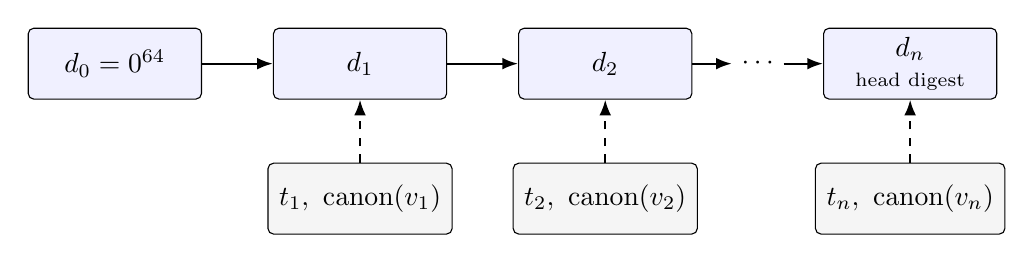
\begin{tikzpicture}[node distance=9mm]
        \node[chain] (d0) {$d_0 = 0^{64}$};
        \node[chain, right=of d0] (d1) {$d_1$};
        \node[chain, right=of d1] (d2) {$d_2$};
        \node[right=5mm of d2] (dots) {$\cdots$};
        \node[chain, right=5mm of dots] (dn) {$d_n$\\[-1pt]{\scriptsize head digest}};
        \node[box, below=8mm of d1] (r1) {$t_1,\ \mathrm{canon}(v_1)$};
        \node[box, below=8mm of d2] (r2) {$t_2,\ \mathrm{canon}(v_2)$};
        \node[box, below=8mm of dn] (rn) {$t_n,\ \mathrm{canon}(v_n)$};
        \draw[arr] (d0) -- (d1);
        \draw[arr] (d1) -- (d2);
        \draw[arr] (d2) -- (dots);
        \draw[arr] (dots) -- (dn);
        \draw[darr] (r1) -- (d1);
        \draw[darr] (r2) -- (d2);
        \draw[darr] (rn) -- (dn);
    \end{tikzpicture}
    \caption{The digest chain over the history of one task.}
    \label{fig:digest-chain}
\end{figure}

\paragraph*{Offline check.} The user can download the whole report as a JSON file. A small script recomputes every digest and says which record, if any, does not match, without the application or the network. This does not replace Fabric's own chain of blocks; it gives a person a portable fingerprint of one history.

\section{Frontend}
\label{sec:frontend}

After signing in, a person sees a dashboard with their projects and their role in each (\Cref{fig:ui-dashboard}). The board shows the tasks of a project, read from the ledger, in three columns, and can be filtered by text, assignee, priority and due date (\Cref{fig:ui-board}). The task page shows details, files, comments and the activity list (\Cref{fig:ui-task}), and the ``Verify audit trail'' button shows the result of the check (\Cref{fig:ui-verify}).

\screenshot{images/ui-dashboard.png}{The dashboard with the user's projects and roles.}{fig:ui-dashboard}
\screenshot{images/ui-board.png}{The task board, read from the ledger.}{fig:ui-board}
\screenshot{images/ui-task.png}{The task page with the activity list.}{fig:ui-task}
\screenshot{images/ui-verify.png}{Result of ``Verify audit trail''.}{fig:ui-verify}

Three choices matter. The interface follows the permission rules and explains why an action is not available. The activity list shows for each change what changed, who changed it and when, so the main guarantee of the system is visible to non-technical users. And because a write takes a few seconds, the interface moves a card immediately and confirms in the background, locking the buttons meanwhile so that nothing is sent twice.


\chapter{Results}
\label{ch:results}

This chapter reports the experiments carried out on the prototype and uses them to answer the research questions. ChainBoard was evaluated in four ways. First, every function was exercised on a real Fabric network and the permission rules were tested with every role. Then the audit verification was tested on untouched histories and on reports manipulated on purpose. The speed of the system was measured with a benchmark. Finally, ten people used the prototype in a small user study. \Cref{tab:eval-overview} shows which research question each experiment answers.

\begin{table}[htbp]
    \centering
    \small
    \begin{tabular}{p{1.1cm}p{5.6cm}p{5.4cm}}
        \toprule
        RQ & What was evaluated & Experiment \\
        \midrule
        RQ1 & The project management functions & Scenarios on the real network, automated tests \\
        RQ2 & Permissions enforced by the chaincode & Every action tried with every role \\
        RQ3 & Verifiable audit trail & Untouched and manipulated histories \\
        RQ4 & Cost and limits & Benchmark, threat model \\
        RQ1, RQ3 & Whether people can use the board and understand the history check & User study with ten participants \\
        \bottomrule
    \end{tabular}
    \caption{Overview of the evaluation.}
    \label{tab:eval-overview}
\end{table}

\section{Setup}
\label{sec:results-setup}

All experiments were run on one machine hosting the Fabric test network (two organizations with one peer each, one orderer and one channel), a local IPFS node, the backend and the frontend. \Cref{tab:environment} lists the details. The machine is an ordinary laptop, not a server, which matters when reading the performance figures. The demonstration data was loaded with a seed script that creates five accounts (an owner, an administrator, two contributors and an outsider), four projects and their tasks, all through the normal API, so that every record is a real transaction.

\begin{table}[htbp]
    \centering
    \small
    \begin{tabular}{ll}
        \toprule
        Item & Value \\
        \midrule
        CPU & Intel Core i5-1335U (13th gen), 12 logical CPUs \\
        RAM available to WSL & 7.6\,GiB \\
        Operating system & Windows 11, WSL2 with Ubuntu 24.04.1 LTS \\
        Docker, Node.js & 26.0.0, 20.20.2 \\
        Hyperledger Fabric & 2.5.16 \\
        Peers, orderers & 2 peers (one per organization), 1 orderer \\
        Batch timeout of the orderer & 2\,s (test network default) \\
        IPFS (Kubo) & 0.29.0 \\
        \bottomrule
    \end{tabular}
    \caption{Test environment.}
    \label{tab:environment}
\end{table}

\section{Functional Evaluation}
\label{sec:results-functional}

The chaincode functions were first called directly with the Fabric peer command-line tool, without the backend, and the same steps were then repeated through the web interface. \Cref{tab:scenarios} lists the scenarios and their outcome. All of them behaved as expected, and the state reached through the interface was the same as the state reached with the command-line tool, so the backend introduces no differences of its own.

\begin{table}[htbp]
    \centering
    \small
    \begin{tabular}{p{0.6cm}p{5.4cm}p{5.0cm}p{0.9cm}}
        \toprule
        \# & Scenario & Observed & Result \\
        \midrule
        F1 & Create a project & Owner is the only member, status \texttt{active} & pass \\
        F2 & Add a member with a role & Member appears in the project with that role & pass \\
        F3 & Create a task & Status \texttt{todo}, no assignee & pass \\
        F4 & Assign the task to a member & Assignee stored; a non-member is refused & pass \\
        F5 & Move the task \texttt{todo}\,$\rightarrow$\,\texttt{in-progress}\,$\rightarrow$\,\texttt{done} & Each move stored and visible on the board & pass \\
        F6 & Jump \texttt{todo}\,$\rightarrow$\,\texttt{done} & Refused as an invalid transition & pass \\
        F7 & Comment on the task & Comment stored with its author & pass \\
        F8 & Attach a file & File uploaded to IPFS, CID stored on the ledger, same file returned by the gateway & pass \\
        F9 & Archive the task and the project & Removed from the board; archived project accepts no new tasks & pass \\
        F10 & Read the history of the task & Every version, oldest first, with author and time & pass \\
        F11 & Sign up, sign in, change password & Account events stored as transactions & pass \\
        \bottomrule
    \end{tabular}
    \caption{Functional scenarios, run on the real network.}
    \label{tab:scenarios}
\end{table}

\section{Permissions}
\label{sec:results-permissions}

To check the permission rules, each action was tried with each of the five seeded accounts, both through the interface and directly against the API, where the interface cannot hide a button. \Cref{tab:perm-results} shows the outcome. Every forbidden action was refused by the chaincode with ``Permission denied'', which the backend returns as HTTP 403, and nothing was written to the ledger. Every allowed action succeeded.

\begin{table}[htbp]
    \centering
    \small
    \begin{tabular}{p{4.6cm}cccc}
        \toprule
        Action & Owner & Admin & Contributor & Outsider \\
        \midrule
        Add a contributor & yes & yes & 403 & 403 \\
        Add an admin & yes & 403 & 403 & 403 \\
        Archive the project & yes & 403 & 403 & 403 \\
        Create a task, comment & yes & yes & yes & 403 \\
        Take a free task & yes & yes & yes & 403 \\
        Assign a task to someone else & yes & yes & 403 & 403 \\
        Change a task assigned to another person & yes & yes & 403 & 403 \\
        Archive a task & yes & yes & 403 & 403 \\
        \bottomrule
    \end{tabular}
    \caption{Outcome of each action for each role (yes = allowed and committed, 403 = refused by the chaincode).}
    \label{tab:perm-results}
\end{table}

Two more checks concern the acting person. A request whose body names a different person is still recorded under the signed-in user, because the backend ignores that field. A call that reaches the chaincode without any acting person is refused by the chaincode itself. Refused calls leave nothing in the history. This is by design: the history records changes, not attempts.

\section{Audit Trail Verification}
\label{sec:results-audit}

The audit verification is the main contribution of the thesis, so it was tested in two situations: on real histories that nobody had touched, and on downloaded reports that were changed on purpose.

On untouched data, ``Verify audit trail'' was run on every task and project of the demonstration data. Each time, all records were found in committed blocks, and the offline verifier computed from the downloaded file the same head digest that the application had shown.

\Cref{tab:tamper} shows the manipulations. In every case the change was detected, and the verifier named the first record that no longer matched. The last row matters too: when the peer could not be reached, the records were marked ``not checked'' instead of ``missing'', so a network problem is not mistaken for tampering.

\begin{table}[htbp]
    \centering
    \small
    \begin{tabular}{p{4.6cm}p{2.0cm}p{5.0cm}}
        \toprule
        Change made to the report or history & Detected & What the user sees \\
        \midrule
        None (untouched history) & -- & Verified, same head digest online and offline \\
        Edit one field of one record & yes & Digest mismatch from that record on \\
        Delete a record & yes & Digest mismatch from the gap on \\
        Swap two records & yes & Digest mismatch from the first swapped record \\
        Insert a fake record & yes & Digest mismatch at the fake record, every later record out of order, record count wrong \\
        Transaction unknown to the peer & yes & Record reported as missing \\
        Peer not reachable & -- & Records reported as not checked \\
        \bottomrule
    \end{tabular}
    \caption{Manipulations of an audit report and the result of the verification.}
    \label{tab:tamper}
\end{table}

As a concrete example, the report of a demonstration task with four records was downloaded, and the offline verifier accepted it unchanged. A copy of the first record with a different transaction identifier was then inserted into the file. The verifier rejected the modified file: the digest of the fake record did not match, every record after it was out of order, and the record count no longer matched.

What the check cannot show is also important. It proves that the history was not changed after it was written. It does not prove that the person recorded in it was really the person who acted, because the backend reports who is acting.

\section{Automated Tests}
\label{sec:results-tests}

The backend tests run the real chaincode on an in-memory implementation of the Fabric interface, behind the real Express application, so they need no network. The frontend tests check the decision logic of each screen without a browser. \Cref{tab:tests} gives the numbers; all 278 tests pass.

\begin{table}[htbp]
    \centering
    \small
    \begin{tabular}{p{7.4cm}rr}
        \toprule
        Area & Tests & Passed \\
        \midrule
        Projects, tasks, transitions, ownership from the session & 18 & 18 \\
        Permissions (every role and action) & 14 & 14 \\
        History, digest chain and audit verification & 17 & 17 \\
        Accounts: sign-up, sign-in, sessions, passwords, Google, e-mail & 98 & 98 \\
        Security: CSRF, headers, route protection, rate limits, bad input & 24 & 24 \\
        Benchmark statistics helpers & 5 & 5 \\
        \midrule
        Backend total & 176 & 176 \\
        Frontend decision logic (14 files) & 102 & 102 \\
        \midrule
        Total & 278 & 278 \\
        \bottomrule
    \end{tabular}
    \caption{Automated tests (Node.js test runner; backend about 8\,s, frontend under 1\,s).}
    \label{tab:tests}
\end{table}

Tests on a simulated ledger are useful for the business rules, but they do not replace running on the network: the order and the field names of the history returned by the real Fabric library differ from those of the in-memory implementation, and this difference became visible only on the real network.

\section{Performance}
\label{sec:results-performance}

The benchmark script sends real requests through the backend, so every write goes through endorsement, ordering and commit. It uses its own temporary account and project. It measures single writes (40 \texttt{createTask} calls one after the other), write throughput with 1, 2, 4 and 8 concurrent clients, contention (8 clients editing the same task at once) and reads (200 reads of one task and of all tasks of a project). The benchmark was run three times in a row, and the tables report, for each value, the median of the three runs. The runs differed very little: write latencies by less than 2\%, reads by a few milliseconds.

\begin{table}[htbp]
    \centering
    \small
    \begin{tabular}{lrrr}
        \toprule
        Operation & p50 (ms) & p95 (ms) & Failed \\
        \midrule
        Write one task (\texttt{createTask}) & 2087 & 2129 & 0 / 40 \\
        Read one task & 30 & 44 & 0 / 200 \\
        Read all tasks of a project & 30 & 57 & 0 / 200 \\
        \bottomrule
    \end{tabular}
    \caption{Latency of single operations through the whole stack (median of three runs).}
    \label{tab:benchmark}
\end{table}

\begin{table}[htbp]
    \centering
    \small
    \begin{tabular}{rrrr}
        \toprule
        Concurrent clients & Throughput (tx/s) & p50 (ms) & p95 (ms) \\
        \midrule
        1 & 0.48 & 2076 & 2099 \\
        2 & 0.95 & 2101 & 2124 \\
        4 & 1.89 & 2116 & 2142 \\
        8 & 3.73 & 2143 & 2172 \\
        \bottomrule
    \end{tabular}
    \caption{Write throughput with concurrent clients writing different tasks.}
    \label{tab:throughput}
\end{table}

\paragraph*{Writes and reads.} A write takes about 2.1 seconds, and the spread is very small: the slowest of 40 writes took 2.16 seconds. Almost all of this time is waiting. When there are only a few transactions, the orderer of the test network cuts a block every 2 seconds, so a write costs the batch timeout plus about 100\,ms for endorsement, validation and commit. Reads take about 30\,ms, around 70 times faster, because one peer answers from its local state without waiting for a block. With the small amount of data used here, reading all tasks of a project costs the same as reading one task.

\paragraph*{Throughput.} Throughput doubles every time the number of clients doubles, from 0.48 to 3.73 transactions per second, while the latency of each write stays almost the same (from 2.08 to 2.14 seconds). The reason is that all writes sent within the same 2-second window end up in the same block. With 8 clients the system had not reached its limit yet; at this load, the block timeout, not the processor, decides the speed.

\paragraph*{Contention.} When 8 clients edited the same task at once, only 1 edit was committed and the other 7 were rejected with an MVCC read conflict, in all three runs. The backend returns these as HTTP 409 so that the user can try again. This is the correct behavior of Fabric: only one change to a key can win in each block. It is also the reason why the data model gives every task, project and account its own key, so that people working on different tasks never block each other.

\paragraph*{How to read these numbers.} Everything ran on one machine, with the load generator sharing the processor with the network, so the figures show orders of magnitude, not the limits of Fabric. They are in line with the factors identified by \textcite{thakkar2018performance}, mainly the block settings of the orderer and conflicts on the same key. A conventional database behind the same API would be faster; the extra time is the price of a history that no single administrator can rewrite. The 2-second wait could be shortened by lowering the batch timeout, at the cost of more and smaller blocks. For a team tool, where a person changes a task every few minutes, a write time of about 2 seconds is noticeable but acceptable, especially because the interface updates the card immediately and confirms in the background.

% NOT included in main.tex yet. After the user test, paste this section back
% into chapters/results.tex, just before \section{Threat Model}.

\section{User Study}
\label{sec:results-usability}

To find out whether people can actually use ChainBoard and understand its audit check, I ran a small usability study.

\paragraph{Participants and procedure.} \textit{tbd} people took part (\textit{tbd} students and \textit{tbd} developers; \textit{tbd} had used Trello or Jira before, \textit{tbd} had used a blockchain application). Each session took about 25 minutes on my laptop. Participants followed a printed sheet of 12 tasks in a prepared project (\Cref{tab:usability-tasks}) and were asked to think aloud. I did not help unless someone was stuck for more than two minutes, which I counted as a failure. Afterwards they filled in the System Usability Scale (SUS)~\cite{brooke1996sus} and two extra statements about the audit trail, on the same 1--5 scale, plus three open questions.

\begin{table}[tb]
    \centering
    \small
    \begin{tabular}{p{0.5cm}p{6.6cm}rr}
        \toprule
        \# & Task & Success & Median time (s) \\
        \midrule
        T1 & Sign in & \textit{tbd}/\textit{n} & \textit{tbd} \\
        T2 & Open the project and its board & \textit{tbd}/\textit{n} & \textit{tbd} \\
        T3 & Find the overdue task & \textit{tbd}/\textit{n} & \textit{tbd} \\
        T4 & Assign it to yourself & \textit{tbd}/\textit{n} & \textit{tbd} \\
        T5 & Move it to In progress & \textit{tbd}/\textit{n} & \textit{tbd} \\
        T6 & Add a comment & \textit{tbd}/\textit{n} & \textit{tbd} \\
        T7 & Create a task with priority and due date & \textit{tbd}/\textit{n} & \textit{tbd} \\
        T8 & Attach a file & \textit{tbd}/\textit{n} & \textit{tbd} \\
        T9 & Mark the task Done & \textit{tbd}/\textit{n} & \textit{tbd} \\
        T10 & Find who completed another task, and when & \textit{tbd}/\textit{n} & \textit{tbd} \\
        T11 & Verify the audit trail and explain the result & \textit{tbd}/\textit{n} & \textit{tbd} \\
        T12 & Try to change another person's task, explain why it fails & \textit{tbd}/\textit{n} & \textit{tbd} \\
        \bottomrule
    \end{tabular}
    \caption{Tasks of the user study, success rate and median completion time.}
    \label{tab:usability-tasks}
\end{table}

\paragraph{Task success.} \ag{Two or three sentences: overall success rate, which tasks were hardest and why (use what people said while thinking aloud).} For T11 and T12 a task counted as successful only if the participant could also explain the result in their own words, for example that the history is stored on a ledger and cannot be changed, or that only the assignee may change a task.

\paragraph{SUS score.} Each SUS answer was converted to a 0--100 score in the standard way: for odd items subtract 1 from the answer, for even items subtract the answer from 5, add the ten values and multiply by 2.5. \Cref{tab:sus} gives the results. An average SUS score is around 68~\cite{lewis2018sus}, so \ag{compare the mean with 68 in one sentence}.

\begin{table}[tb]
    \centering
    \small
    \begin{tabular}{lrrrr}
        \toprule
        Measure & Mean & SD & Min & Max \\
        \midrule
        SUS score (0--100) & \textit{tbd} & \textit{tbd} & \textit{tbd} & \textit{tbd} \\
        ``I understood what the result of Verify audit trail means'' (1--5) & \textit{tbd} & \textit{tbd} & \textit{tbd} & \textit{tbd} \\
        ``Being able to check a task's history makes me trust it more'' (1--5) & \textit{tbd} & \textit{tbd} & \textit{tbd} & \textit{tbd} \\
        \bottomrule
    \end{tabular}
    \caption{Questionnaire results ($n = \textit{tbd}$).}
    \label{tab:sus}
\end{table}

\paragraph{What participants said.} \ag{Summarize the open answers and think-aloud notes in a short paragraph or a small table: the two or three most common problems, what people liked, and one or two short quotes.}

\paragraph*{Changes made after the first session.} The study was used to improve the prototype while it was running. In the first session, the participant did not find how to set the priority and the due date of a new task (T7): the create-task bar showed only a title field and an ``Add task'' button, and the other fields were hidden behind a small ``More options'' link. After this session the create-task card was redesigned. The board now shows a single ``Add new task'' button, which opens a card that has a heading, a labelled title field, the priority as three visible buttons (low, medium, high), a visible due-date field, an optional description, and a ``Create task'' button with a hint when the title is missing; the task identifier is always generated automatically and is no longer shown. The result of the audit verification was also rewritten in plain language. The button ``Verify audit trail'' became ``Check that this history is genuine'', with one sentence explaining what it does; the result says, for example, ``This history is genuine: all 3 changes were found in the blockchain exactly as they are shown here'', the head digest is shown as a ``history code'' with a short explanation, and transaction identifiers moved under ``Technical details''. The following sessions used the new version. \ag{Say how many sessions used the old and the new version, and whether T7 became easier.}

\paragraph*{Changes made after the second session.} \ag{Start with what you observed in session 2 that led to these changes, e.g. where the participant got lost or hesitated.} After the second session the layout of the application was reorganized. A sidebar now lists the person's projects, so switching project takes one click from anywhere, and each project has a header with two tabs, ``Board'' and ``Members and history'', instead of separate pages and a ``Project settings'' button. A task no longer opens on its own page: it opens in a window over the board, with the status as three buttons under the title, a single line with priority, due date, assignee and task identifier, and below it the description, files, comments and activity. The separate ``Edit'' mode was removed; title, description, priority and due date are now changed in place and each change is saved as its own transaction. When a person tries to change something they are not allowed to, for example a task assigned to someone else, or to archive a task without being owner or admin, the interface now explains why instead of silently ignoring the click; the chaincode still enforces the same rules. Finally, the light theme was changed from grey to a warm off-white with near-black text and all text colours at or above the WCAG AA contrast of 4.5:1~\ag{cite WCAG 2.1}. \ag{Say which sessions used this version.}

With \textit{tbd} participants the study cannot give precise numbers, and most participants were students, not professional teams. It does show whether the main ideas, a familiar board and a visible audit check, make sense to people who did not build the system.


\section{Threat Model}
\label{sec:results-threats}

\paragraph*{Trust assumptions.} No single party is assumed to control both endorsement and ordering in the Fabric network. The backend is trusted, because it holds the Fabric identity of the organization, verifies the login session and tells the chaincode who is acting. Browsers are not trusted.

\paragraph*{What the design protects against.} Under these assumptions, an administrator cannot quietly change a status, a due date or a comment, because every change is a new transaction and the old versions stay in the history. A history changed in a copy of the data is detected by the digest chain, also offline. Two accounts cannot share a username, phone number or Google account. A user cannot perform an action that their role forbids, even if the backend has a bug, because the chaincode checks the role on every write.

\paragraph*{What it does not protect against.} \Cref{tab:threats} lists the remaining risks, which set the limits of the claims made in this thesis.

\begin{table}[htbp]
    \centering
    \small
    \begin{tabular}{p{3.4cm}p{8.6cm}}
        \toprule
        Threat & Why it remains, and how it could be fixed \\
        \midrule
        Compromised backend & Fabric only sees the organization, so the chaincode trusts the backend about who is acting. Fix: one Fabric certificate per person. \\
        One organization controls all endorsers & The test network has two organizations but one trust domain. Fix: require both organizations to endorse critical actions. \\
        Stolen password or session & Usual web risk, reduced by scrypt hashing, HttpOnly cookies, rate limits and CSRF checks. \\
        Reading without permission & Reads are not checked by role. Fix: role-checked reads or Fabric private data. \\
        Lost attachments & The CID proves what a file contained, but nobody is obliged to keep the file. Fix: pinning. \\
        Personal data on the ledger & Ledger data cannot be erased, which conflicts with the GDPR right to erasure~\cite{gdpr}. Fix: keep personal data off-chain and store only hashes. \\
        \bottomrule
    \end{tabular}
    \caption{Remaining threats.}
    \label{tab:threats}
\end{table}

\section{Support for Scrum and Kanban}
\label{sec:results-agile}

ChainBoard is in practice a Kanban board with a verifiable history. It does not implement Scrum; this was left out on purpose, because the research questions concern the integrity of the record, not planning features. \Cref{tab:agile} shows what is covered.

\begin{table}[htbp]
    \centering
    \small
    \begin{tabular}{p{4.4cm}p{1.6cm}p{6.0cm}}
        \toprule
        Element & Supported & Comment \\
        \midrule
        Board with workflow columns & yes & To do, in progress, done \\
        Tasks with priority, due date, assignee, comments, files & yes & \\
        Product backlog & partly & A flat list of tasks, no ordering \\
        Sprints, sprint goal & no & \\
        Scrum roles & no & Owner, admin and contributor only control permissions \\
        Estimation, burndown, velocity & no & \\
        Work-in-progress limits & no & \\
        Verifiable history of every change & yes & Not offered by Trello, Jira or similar tools \\
        \bottomrule
    \end{tabular}
    \caption{Scrum and Kanban elements in ChainBoard.}
    \label{tab:agile}
\end{table}

The history is still useful for Scrum events that the tool does not support directly. In a sprint review or retrospective, the team can see exactly when each task moved and who moved it, and a task that was reopened cannot be hidden.

\section{Answers to the Research Questions}
\label{sec:rq-answers}

\textbf{RQ1.} Yes. The Fabric-plus-IPFS pattern carries over to software project management with a different data model (users, projects, tasks, comments and attachments, with keys designed for a store that has no queries by field value) and a familiar board workflow. All eleven functional scenarios of \Cref{tab:scenarios} passed on the real network, through the command-line tool and through the web interface.

\textbf{RQ2.} Yes, with one qualification. In the permission experiment every forbidden action was refused by the chaincode, also when the API was called directly and the interface was bypassed, and refused calls left no trace on the ledger (\Cref{tab:perm-results}). The qualification is that the chaincode learns \emph{who} is acting from the backend, because Fabric authenticates the organization and not the person. Closing this gap requires one Fabric identity per person.

\textbf{RQ3.} The system checks every transaction against the peer, computes a digest chain over the history, and lets the user download a report that a stand-alone script verifies offline. Every manipulation tried in \Cref{tab:tamper} was detected, and an unreachable peer was never reported as tampering. The check shows that a history was not altered; it does not show that the person recorded as acting was really the one who acted.

\textbf{RQ4.} A write costs about 2.1 seconds, almost all of it waiting for the orderer to cut a block, while a read costs about 30\,ms. Throughput grew linearly from 0.48 to 3.73 transactions per second between 1 and 8 clients, and of 8 simultaneous edits of the same task only one was committed. The limits are those of \Cref{tab:threats}: identity, confidentiality of reads, permanence of personal data, availability of attachments, and the scale of the evaluation.

\section{Discussion}
\label{sec:results-discussion}

The experiments give a consistent picture. The functions that a software team expects from a board are available and behave the same through the interface and directly on the chaincode; the permission rules hold even when the interface is bypassed; and every manipulation of a history was detected, also offline. The price is speed: a write takes about two seconds instead of the few milliseconds of a conventional database, because it waits for a block. For the intended use, a team tool where each person changes a task every few minutes, this cost is acceptable.

Two observations go beyond the numbers. A test setup that simulates the ledger can differ from the real library in ways that hide defects, so tests on the real network remain necessary. And the most important limitation is architectural: because the Fabric gateway identifies an organization and not a person, a rule such as ``only an owner may archive a project'' holds only as far as the backend that reports who is acting can be trusted. The evaluation also used a local network with two organizations, not a geographically distributed or production-scale deployment; \Cref{ch:conclusion} discusses the consequences as limitations and future work.


\chapter{Conclusion}
\label{ch:conclusion}

This thesis addressed one limitation of the software project management platforms in wide use today: because a single provider stores and controls the history of a project, nobody else can verify that the history has not been tampered with. Starting from the architectural pattern validated for decentralized data management in the construction industry~\cite{adel2023}, the thesis adapted that pattern to software project management and implemented it in a working prototype, ChainBoard.

ChainBoard models accounts, projects and tasks as chaincode-governed state on a permissioned Hyperledger Fabric network. Its operations for creating projects, managing membership and roles, assigning tasks, changing status, commenting and archiving are all recorded in the immutable transaction history of Fabric, not in a log controlled by a provider. The chaincode itself decides who may do what, from the roles stored in the project, so the permission rules do not depend on the backend or the user interface. File attachments are stored on IPFS and anchored to the ledger by their CIDs, which keeps binary data off the chain while still tying each recorded reference to the exact file content. A backend API and a browser frontend offer these functions through a task board similar to Trello or Jira. The audit trail, the main guarantee of the system, is visible and can be checked: every change shows who made it and when, and a verification step checks each record against the ledger and produces a downloadable report with a digest chain that can be verified again offline.

The experiments of \Cref{ch:results} support these claims with concrete results. All eleven functional scenarios passed on a real Fabric network; every forbidden action was refused by the chaincode, also when the interface was bypassed; every manipulation of an audit report was detected; and all 278 automated tests pass. The cost of the guarantee is about two seconds per write, while a read takes about 30 milliseconds. In the user study, all ten participants completed every task and the interface scored 86 on the System Usability Scale. Overall, the Fabric-plus-IPFS pattern carries over to software project management with the same architecture; what changes is the data model and the workflow offered to users.

\section{Limitations}
\label{sec:limitations}

The prototype was evaluated on a local Fabric network with two organizations, not on a geographically distributed or production-scale deployment. The performance figures describe one machine under a synthetic load, not realistic use by many people, and they include no comparison with a conventional database. The most important limitation is the identity model. The Fabric gateway authenticates the organization and not each person, so the backend authenticates people with its own login sessions and tells the chaincode who is acting. The chaincode enforces the \emph{rules} but has to trust the backend about \emph{who} is acting, and a compromised backend could claim any identity. Reads are not restricted by role, so any signed-in person who knows a project identifier can read it. Data written to the ledger is permanent, which conflicts with the right to erasure of the GDPR~\cite{gdpr} for personal data such as names and comments. Attachments are anchored by CID, but nothing in the prototype guarantees that the files stay available. Finally, the data model is deliberately small. It supports a Kanban-style board but not the Scrum framework (there is no backlog ordering, no sprints, no estimation and no burndown chart), and it does not yet cover sub-tasks, dependencies between tasks, notifications or access control per field.

\section{Future Work}
\label{sec:future-work}

The limitations above suggest several directions. The most useful is to give every person their own Fabric identity, with a certificate issued by the Fabric certificate authority, so that the chaincode reads the caller from the client identity of the transaction instead of trusting the backend, as the Fabric-based tool of \textcite{batista2021} already does, and to require endorsement by both organizations for critical actions such as archiving a project. Attribute-based policies of the kind studied by \textcite{gordijn2022combining} could then express the project roles directly in the certificates. Restricting reads by role, or placing sensitive fields in Fabric private data collections and keeping personal data off-chain with only hashes on the ledger, would address confidentiality and erasure. Evaluating the system on a geographically distributed network with a realistic number of organizations and peers, and comparing it with a conventional database, would show its throughput and latency under conditions closer to production. The user study showed that participants value a verifiable history but do not always understand the result of the manual check, so the check could run automatically in the background and show only its outcome, without technical terms; a longer study with real teams over several weeks would also show how the tool is used in practice. Extending the data model with sprints, a backlog, story points, burndown charts, sub-tasks, dependencies and notifications would close the functional gap with mature centralized platforms while keeping the same audit guarantees, and pinning attachments, with a check of the CID on download, would make file storage as dependable as the ledger. Finally, the architectural pattern is not specific to software projects, and applying it to other collaborative domains that need a verifiable history would show how far it generalizes.


\appendix
\crefalias{chapter}{appendix}
\chapter{Reproducing the Prototype and its Evaluation}
\label{app:reproduce}

This appendix lists the steps needed to run the prototype and repeat the measurements of \Cref{ch:results}. The source code is in the repository named in the project README; the commands assume Linux or WSL2 with Docker, Node.js 20.9 or newer, and the Hyperledger Fabric binaries and \texttt{test-network} of the \texttt{fabric-samples} repository.

\section{Starting the Network and the Application}
\label{app:start}

\begin{lstlisting}[numbers=none, language={}, basicstyle=\ttfamily\footnotesize]
cd ~/fabric-samples/test-network
./network.sh down
./network.sh up createChannel -c mychannel
./network.sh deployCC -ccn pmcc -ccp ../dpm-project/pm-chaincode \
    -ccl javascript -ccv 1.0 -ccs 1

cd ~/fabric-samples/dpm-project/pm-backend  && npm install && npm run dev
cd ~/fabric-samples/dpm-project/pm-frontend && npm install && npm run dev
\end{lstlisting}

The chaincode functions changed signature when permissions were added, so after any chaincode change it is simplest to recreate the network with \texttt{./network.sh down}. Demonstration data (five accounts, four projects and their tasks) can be loaded with \texttt{npm run seed} in the backend folder.

\section{Tests and Benchmark}
\label{app:tests}

\begin{lstlisting}[numbers=none, language={}, basicstyle=\ttfamily\footnotesize]
cd pm-backend  && npm test            # backend suite, no network needed
cd pm-frontend && npm test            # frontend decision logic
cd pm-backend  && npm run benchmark   # needs the running network and backend
npm run verify-audit -- audit-task-<id>.json   # offline check of a report
\end{lstlisting}

The benchmark writes its measurements to \texttt{benchmark-results.json} and \texttt{benchmark-results.csv}, from which \Cref{tab:benchmark} is filled in.

\section{Summary of the REST API}
\label{app:api}

\Cref{tab:api} lists the main endpoints. All endpoints other than sign-in and sign-up require a valid session cookie, and state-changing requests are checked against the \texttt{Origin} and \texttt{Host} headers.

\begin{table}[tb]
    \centering
    \small
    \begin{tabular}{p{1.3cm}p{5.6cm}p{5.4cm}}
        \toprule
        Method & Path & Chaincode function \\
        \midrule
        POST & \texttt{/api/projects} & \texttt{createProject} \\
        POST & \texttt{/api/projects/\{id\}/members} & \texttt{addProjectMember} \\
        DELETE & \texttt{/api/projects/\{id\}} & \texttt{archiveProject} \\
        GET & \texttt{/api/projects/\{id\}/tasks} & \texttt{getProjectTasks} \\
        GET & \texttt{/api/projects/\{id\}/audit} & \texttt{getProjectHistory} + ledger check \\
        POST & \texttt{/api/tasks} & \texttt{createTask} \\
        PUT & \texttt{/api/tasks/\{id\}/assign} & \texttt{assignTask} \\
        PUT & \texttt{/api/tasks/\{id\}/status} & \texttt{updateTaskStatus} \\
        PUT & \texttt{/api/tasks/\{id\}/meta} & \texttt{updateTaskMeta} \\
        POST & \texttt{/api/tasks/\{id\}/comments} & \texttt{addComment} \\
        POST & \texttt{/api/tasks/\{id\}/files} & \texttt{attachFile} \\
        DELETE & \texttt{/api/tasks/\{id\}} & \texttt{archiveTask} \\
        GET & \texttt{/api/tasks/\{id\}/audit} & \texttt{getTaskHistory} + ledger check \\
        \bottomrule
    \end{tabular}
    \caption{Main REST endpoints and the chaincode functions they invoke.}
    \label{tab:api}
\end{table}


% Bibliography using biber; comment this and uncomment the following lines to use bibtex instead
\printbibliography
% \bibliographystyle{alphaurl}
% \bibliography{bib}

\end{document}

